
%\subsection{Computation pipeline}
\section{The Probabilistic Trace Alignment Tool}
%We now describe the proposed technique for computing probabilistic trace alignments.
Our tool takes as input
\begin{inparaenum}[\it (i)]
	\item a reference model represented as a BPMN model or an equivalent stochastic Workflow net,
	\item a minimum positive probability threshold $\pmin \in (0,1]$
	\item a trace $\trace$ of interest,
\end{inparaenum}
and returns a ranking over all the model traces having a probability greater than or equal to $\pmin$, based on a combined consideration of their probability values and their distance from $\trace$.

%\begin{figure}[!t]
%	\centering
%	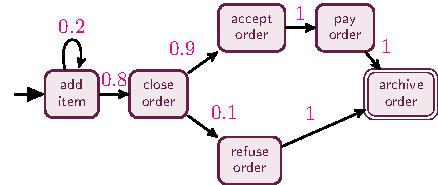
\includegraphics[width=.4\textwidth]{images/besser_rg}
%	\caption{Transition Graph for \figurename~\ref{fig:bpmn-order}.}
%\end{figure}
\medskip
\noindent
\textbf{Transition Graphs.} The model trace probabilities can be directly computed by inspecting the reachability graph of the reference model. Still, graph embedding techniques required to represent traces as data points (e.g., vectors)
cannot be directly defined over reachability graphs as they %. In fact, these techniques
rely on probabilistic \emph{Transition Graphs} \cite{GartnerFW03}. Such Transition Graphs can be computed by firstly shifting the transition labels over graph nodes, and performing $\tau$-closures, while preserving $\tau$-transitions for both start and completion nodes, if required, to preserve trace probabilities. An example of a Transition Graph is shown in \figurename~\ref{fig:closedd}.
%The resulting graphs are described by transition probabilities in a matrix $R$, while nodes are associated to their labels via a matrix $L$, while the same label may be used for multiple nodes. $R$ is then a probability distribution over the next nodes to be picked upon executing a transition.
%A special combination of matrices $L$ and $R$ describes the probability of reaching a node labeled by $\beta$ from any node labeled $\alpha$ in $n$ steps \cite{GartnerFW03}. Model traces are defined similarly from \uswn{s}. This gives us a direct way
%Our untimed, stochastic Workflow nets with bounded silence enjoy the following property: given a net with a bound $b$ on the maximum number of consecutive silent transitions and a model trace of length $n$, a model run yielding that trace must have a length bounded by $n+(n+1)\cdot b$.
%This gives us a direct way to compute the probability of a model trace of a stochastic Workflow net or of an equivalent Transition Graph:
%\begin{enumerate}
%	\item  we fetch all model runs of length at most $n+(n+1)\cdot b$ (which can be easily done with a bounded-depth search strategy over reachable markings);
%	\item among all such runs, we keep all and only those that yield the model trace of interest;
%	\item we sum up the probabilities of the so-filtered model runs.
%\end{enumerate}


\medskip
\noindent
\textbf{Alignment Strategies.}\label{subsec:as}
%Our technique is realized through the pipeline shown in \figurename~\ref{fig:pipe}, consisting of the following steps.
%
%In step 1, the reachability graph $\rg{\net}$ of $\net$ is constructed.
%
%In step 2,
%$\closed{\tg_{\rg{\net}}}$ preserves model traces and their probabilities while working only over visible tasks in $\tasks$;
% this transition graph is unraveled c we apply a probabilistic alignment technique that ranks all such model traces according to their probability and their similarity to $\trace$.
%
%The pipeline has the following phases: after representing the USWN as a graph of all the sequentially scheduled transitions
%(\S\ref{sec:seqZ}), we shift the labels from the edges towards the nodes while preserving the set of probabilistic traces
%(\S\ref{sec:LSift}) and minimize the graph representation by removing the $\tau$-labeled nodes while preserving the
%trace probability (\S\ref{sec:clos}).
%The last step takes the so-obtained model traces and ranks the best $k$ by considering their probabilities and the alignment cost with the trace $\trace$ of interest. %In \figurename~\ref{fig:pipe}, this is shown as a black-box. %As we describe in detail next, we have implemented this last step in two alternative ways: one computationally demanding but guaranteeing to produce an optimal ranking, the other more efficient but providing approximate ranking without optimality guarantees.
%\todo{Ho tagliato la descrizione che c'era dopo. Al limite la incorporerei nella rispettiva sottosezione.}
%We later discuss how to rank traces in the exact and approximated scenarios by reducing the alignment process to a k-nearest
%neighbour problem. While the exact trace alignment requires to perform the alignment process each time a novel trace $\sigma^*$ is
%introduced (\S\ref{subsec:exbkptap}), the approximated alignment can split the alignment into a preliminary loading phase and a
%query phase. In the former, each stochastic trace from the USWN is represented as a vector (\S\ref{subsec:ate}), and in the latter the to-be-aligned trace $\sigma^*$ is first represented as a vector and then compared to all the other vectorial representations.